% le caratteristiche richieste dall'università sono elencate qui: https://stem.elearning.unipd.it/mod/book/view.php?id=234&chapterid=46#modalita
% 12pt: font richiesto dall'università
% twoside: i margini interni ed esterni sono scambiati per le pagine "a sinistra" e "a destra"
% openright: i capitoli cominciano in pagine dispari ("a destra")
% extreport: supporta 12pt
\documentclass[12pt,a4paper,twoside,openright]{extreport}

\usepackage{amsmath}                            % per avere più controllo sulle equazioni 
\usepackage{csquotes}                           % per le citazioni
\usepackage{enumitem}                           % per avere più controllo sulle enumerazioni
\usepackage[
    a4paper,
    top=2cm,bottom=2cm,
    outer=2cm,inner=3cm,
    includeheadfoot
]{geometry}                                     % margini richiesti dall'università
\usepackage{graphicx}                           % per le immagini
\usepackage{icomma}                             % per separare le cifre decimali con una virgola
\usepackage{minted}                             % per il codice con la colorazione della sintassi
\usepackage[a-1a]{pdfx}                         % formato richiesto dall'università
\usepackage[output-decimal-marker={,}]{siunitx} % per le unità di misura
\usepackage{subcaption}                         % per le sottodidascalie
\usepackage{svg}                                % per inserire file SVG

\usepackage[italian]{babel}
\selectlanguage{italian}

\usepackage[backend=bibtex,style=ieee]{biblatex}
\bibliography{bibliografia}

\usepackage{fontspec}
\setmainfont{Times New Roman} % carattere richiesto dall'università

\usepackage{setspace}
\onehalfspacing % interlinea richiesta dall'università

\sloppy % per evitare che il testo in \verb finisca oltre i margini

% questi valori vengono usati nella composizione del frontespizio
\title{Blockchain e Learning Analytics: Una Nuova Frontiera per la Gestione dei Dati}
\author{Speranza Ludovico}
\date{GG/MM/AAAA}
\newcommand{\supervisor}{Prof. Varagnolo Damiano}
\newcommand{\assistantsupervisor}{Cognome Nome}
\usepackage{wrapfig}
\usepackage{float}

\begin{document}
    \pagenumbering{roman}
    \pagestyle{empty} % per le prime pagine, non mostrare il numero di pagina

    \begin{titlepage}
    % solo il frontespizio deve essere simmetrico rispetto ai margini interno ed esterno
    \newgeometry{hmargin=2.5cm,vmargin=2cm}
        \begin{figure}
            \centering
            \begin{subfigure}[b]{0.4\textwidth}
                
\includegraphics[width=\textwidth]{Immagini/logo_unipd}
            \end{subfigure}
            \hfill
            \begin{subfigure}[b]{0.3\textwidth}
                
\includegraphics[width=\textwidth]{Immagini/logo_dei}
            \end{subfigure}
        \end{figure}
    
        \vspace*{\stretch{0.5}}
    
        \begin{center}
            \makeatletter % serve per poter usare \@...

            % NOTA: il Times New Roman non supporta il maiuscoletto.
            \textsc{DIPARTIMENTO DI INGEGNERIA DELL'INFORMAZIONE}\\
            \vspace*{\stretch{0.1}}
            \textsc{CORSO DI LAUREA IN INGEGNERIA INFORMATICA}
    
            \vspace*{\stretch{0.5}}
            \LARGE
            \textbf{\@title}
    
            \vspace*{\stretch{1}}
            \normalsize
            \begin{tabular*}{\textwidth}{l @{\extracolsep{\fill}} r}
                \textbf{Relatore} & \textbf{Laureando} \\
                \supervisor       & \@author           \\
                \\
                %\textbf{Correlatore} \\
                % \assistantsupervisor \\
            \end{tabular*}
    
            \vspace*{\stretch{2}}
            \textsc{ANNO ACCADEMICO 2024-2025} \\
            \vspace*{\stretch{0.1}}
            Data di laurea \@date
        
            \makeatother % serve dopo \makeatletter
        \end{center}
    \restoregeometry
\end{titlepage}

    \cleardoublepage
    
    \vspace*{\stretch{1}}
\begin{flushright}
    \textit{Apes. Together. Strong.}
\end{flushright}
\vspace{\stretch{4}}
    \cleardoublepage

    \pagestyle{plain} % comincia a mostrare il numero di pagina

    % NOTA: l'ambiente \abstract rimuove il numero della pagina e resetta il contatore delle pagine. 
    \chapter*{Abstract}
    La Blockchain è una tecnologia spesso definita "l’Internet del futuro", poiché rappresenta un vero e proprio stravolgimento infrastrutturale con potenziali ripercussioni in numerosi settori. La sua componente innovativa risiede nella possibilità di sviluppare applicazioni decentralizzate e sicure, che non richiedono la presenza di un intermediario. Grazie a queste caratteristiche, la Blockchain è destinata a trasformare molti aspetti della società moderna e si trova oggi al centro di discussioni tecnologiche e monetarie.
    \\Questa tesi esplora l’evoluzione della Blockchain, analizzando inizialmente l’aspetto per cui è nata, ovvero la gestione delle criptovalute, soffermandosi in particolare su Bitcoin ed Ethereum e sui loro algoritmi di validazione. Successivamente, il lavoro si concentra sul tema della protezione dei dati personali, partendo dal Web 3.0 per arrivare ad affrontare le problematiche del Learning Analytics.
    Viene fornita un’analisi critica del sito FaceItTools, proponendo una sua possibile trasformazione blockchain-oriented al fine di migliorare la gestione dei dati, garantendo maggiore trasparenza e affidabilità. In aggiunta, vengono analizzati Blockcerts, EduCTX e Sony Global Education come esempi concreti di piattaforme basate sulla blockchain.  
    \\La ricerca proposta si pone l'obiettivo di offrire una visione completa e critica delle opportunità offerte dalla Blockchain, mettendo in evidenza, in particolare, le potenzialità che essa può avere nel trattamento dei dati sensibili degli studenti in ambito scolastico.
    \cleardoublepage

    \tableofcontents
    \cleardoublepage
    
    \listoffigures
    \cleardoublepage % per assicurarsi che la numerazione araba cominci col primo capitolo
    
    \pagenumbering{arabic}

    \chapter{Blockchain}

Nonostante il grande successo della trasformazione digitale, molti ambiti delle nostre interazioni sono rimasti indietro e non si sono adattati al digitale; un esempio su tutti è quello del settore legale. Inoltre, la digitalizzazione presenta anche lati oscuri \cite{La_quarta_rivoluzione_industriale}: i nostri dati sono controllati da organizzazioni il cui obiettivo principale è il profitto, gli hacker tentano continuamente di sottrarre informazioni personali, e gli Stati monitorano le attività dei cittadini per mantenere l’ordine e il controllo.
\begin{wrapfigure}{r}{0.25\textwidth} %this figure will be at the right
    \centering
    
\includegraphics[width=0.25\textwidth]{Immagini/Satoshi_Nakamoto.jpg}
    \caption{Statua raffigurante Satoshi Nakamoto}
\end{wrapfigure}
Tutto ha origine nel 2008, con la pubblicazione online dell’articolo “Bitcoin: A Peer-to-Peer Electronic Cash System” da parte di Satoshi Nakamoto, pseudonimo che potrebbe celare un individuo o un gruppo di persone. L’obiettivo del documento era quello di creare un sistema puramente peer-to-peer per il trasferimento di valore tra le parti, eliminando la necessità di intermediari come banche o istituti finanziari.
Il concetto chiave della blockchain è la possibilità di creare una generazione di piattaforme decentralizzate e disintermediate, nelle quali la fiducia tra le parti non è garantita da un’organizzazione centrale, ma dalla piattaforma stessa, attraverso un meccanismo algoritmico essa si riferisce, in senso più ampio, all’insieme di tecnologie che rendono possibile la decentralizzazione, basandosi sul modello peer-to-peer, in sostanza consente di immaginare un mondo organizzato in modo completamente diverso.
La blockchain è un database completamente decentralizzato, di cui ogni nodo possiede una replica e concordano, sulla base di un algoritmo comune, un’unica versione aggiornata delle informazioni. Si tratta di una struttura dati nella quale è possibile solo aggiungere nuovi dati, senza possibilità di cancellare quelli precedenti, garantendo così uno storico completo delle modifiche.
Per chiarire meglio questo concetto, possiamo immaginare la blockchain come una barriera corallina: lo strato attivo corrisponde alla parte più recente, che viene continuamente modificata con nuove aggiunte, mentre gli strati più vecchi rimangono immutabili e accessibili solo per attività di consultazione.
Può essere quindi rappresentata come una lista in continua crescita di “blocchi” collegati tra loro e protetti mediante crittografia. Oltre alla decentralizzazione e all’immutabilità, il terzo grande punto di forza è il consenso: nuove transazioni possono essere registrate solo quando la maggioranza dei partecipanti alla rete dà il proprio consenso. \\
I blocchi sopra citati sono composti da 7 campi principali: 
\begin{itemize}
    \item[\textit{Block}:]  rappresenta il numero del blocco all'interno della blockchain. Ogni volta che un nuovo blocco viene aggiunto, questo numero aumenta progressivamente.
    \item[\textit{Nonce}:]  è un valore, spesso composto da 32 bit (come nel caso di Bitcoin), fondamentale perché viene cercato dai miner per generare un hash valido che soddisfi i requisiti di difficoltà della chain. Serve a modificare l’input del calcolo dell’hash e viene aggiornato continuamente durante il processo di mining.
    \item [\textit{Timestamp}:] indica il momento esatto in cui il blocco è stato aggiunto alla blockchain.
    \item [\textit{Transaction}:] contiene o un valore (ad esempio un importo monetario), o il corpo del messaggio, o uno smart contract.
    \item [\textit{Transaction n}:] si riferisce a una specifica transazione tra le diverse transazioni presenti all’interno del blocco.
    \item [\textit{Prev Hash}:] è l’hash del blocco precedente, che funge da chiave di collegamento tra i blocchi. Questo meccanismo garantisce che ogni blocco sia dipendente dal precedente, creando una catena ininterrotta.
    \item [\textit{Hash}:] rappresenta l’impronta digitale del blocco. È un valore alfanumerico unico calcolato applicando una funzione hash. L’hash è deterministico, nel senso che lo stesso input produrrà sempre lo stesso hash; tuttavia, non è possibile risalire ai dati originali partendo dall’hash. Ogni minima modifica ai dati genera un hash completamente diverso, garantendo così l’integrità e l’immutabilità delle informazioni.
\end{itemize}

\begin{figure}[t]
\caption{Esempio di catena}
\centering
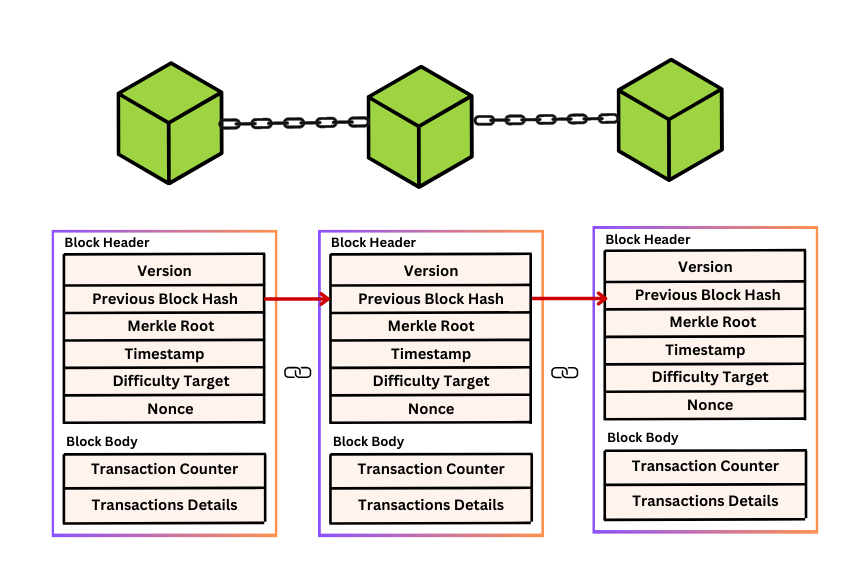
\includegraphics[width=0.8\textwidth]{Immagini/structure of block.png}
\end{figure}

\clearpage

\section{Blokchain 1.0}

\subsection{Bitcoin}

L’aspetto rivoluzionario di Bitcoin è la creazione di una forma monetaria completamente decentralizzata. La sua rete è composta da una serie di componenti chiamate nodi, che collaborano tra loro per raggiungere il consenso su una sequenza di transazioni.
Essendo basato sulla blockchain, Bitcoin è completamente decentralizzato: non è gestito da un’entità centrale, come avviene per esempio con le banche. Questo comporta un vantaggio significativo, ovvero una maggiore resistenza a comportamenti anomali o malintenzionati. In un sistema centralizzato, infatti, il nodo centrale rappresenta un punto di vulnerabilità che potrebbe compromettere l’intero sistema.
Un’altra caratteristica fondamentale di Bitcoin è la disintermediazione: ogni transazione coinvolge direttamente il mittente e il destinatario, che raggiungono il consenso tramite l’approvazione della rete. Bitcoin è quindi costituito da una rete di sistemi indipendenti, i nodi, capaci di mantenere un registro univoco e condiviso delle transazioni. Questo sistema garantisce che un singolo bitcoin non possa essere speso più di una volta.\\
In tal modo, Bitcoin soddisfa le funzioni critiche di ogni valuta:
\begin{itemize}
\item Immagazzinare valore.
\item Essere un’entità contabile.
\item Trasferire valore tra le parti.
\end{itemize}
La sua blockchain è di tipo permissionless, il che significa che chiunque può eseguire il software del nodo e collegarsi alla rete senza alcuna forma di autenticazione. In altre parole, chiunque può unirsi alla rete senza necessità di approvazioni o permessi da parte di un’autorità centrale.
Un elemento fondamentale è il wallet che consente agli utenti di gestire i propri bitcoin, conservati in veri e propri conti. Ogni bitcoin è associato a un address, protetto da una coppia di chiavi crittografiche:
La chiave pubblica rappresenta l’indirizzo del conto ed è accessibile a tutti.
La chiave privata rappresenta l’identità del proprietario ed è necessaria per accedere e autorizzare le transazioni.
Bitcoin utilizza la crittografia asimmetrica, un sistema inventato nel 1976 da Whitfield Diffie e Martin Hellman. Questo metodo permette di cifrare un messaggio con una chiave (pubblica) che può essere decifrato solo con l’altra chiave (privata), e viceversa, ciò determina due vantaggi principali.
Il primo è Hashing dei dati che trasforma qualsiasi quantità di dati in una stringa cifrata di dimensioni fisse, chiamata digest.\\
\\
\\
\\
\\
L’hashing è: 
\begin{itemize}
    \item[\textit{Deterministico}:] ovvero lo stesso input produce sempre lo stesso digest.
    \item [\textit{Lunghezza fissa}:] il digest ha una lunghezza predeterminata, indipendentemente dalla dimensione dell’input.
    \item [\textit{Unico}:] è estremamente improbabile che due input diversi generino lo stesso digest.
    \item [\textit{Non invertibile}:] è impossibile risalire all’input originale partendo dal digest.
    \item [\textit{Instabile}:] una minima modifica all’input genera un digest completamente diverso.
\end{itemize}
Il secondo grosso vantaggio è la firma digitale che garantisce unicità e non ripudiabilità. Quando un utente X invia a un utente Y un messaggio firmato digitalmente, X crea l’hash del messaggio e lo cifra con la propria chiave privata. Y, ricevendo il messaggio, può verificare l’hash con la chiave pubblica di X, garantendo così l’integrità del messaggio e la validità del mittente.
\begin{figure}[h]
\caption{Esempio di cifratura asimettrica}
\centering
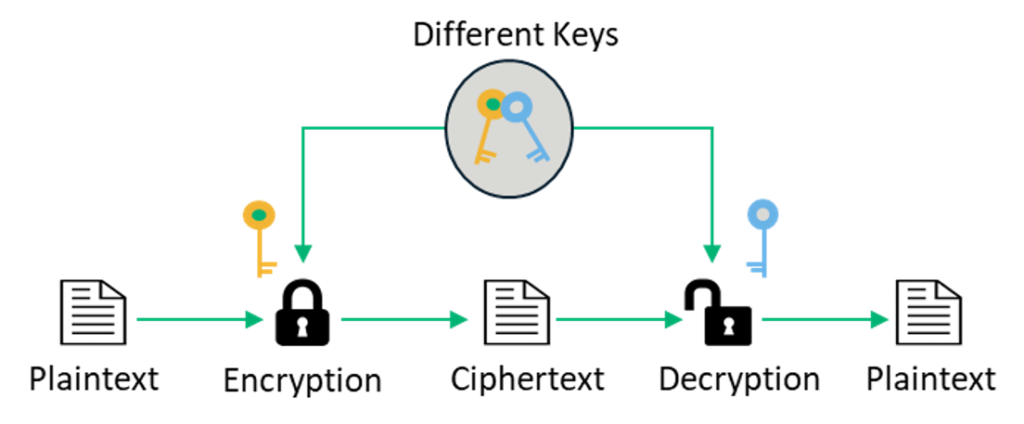
\includegraphics[width=0.65\textwidth]{Immagini/cifratura asimmetrica.png}
\end{figure}
\\
Bitcoin è open source, il suo codice sorgente è pubblico e rilasciato sotto licenza MIT, che permette la massima libertà di utilizzo per progetti futuri.
Nonostante il grande successo riscosso, Bitcoin presenta diverse criticità che ne limitano l'efficacia e l'adozione su larga scala. Una delle principali problematiche riguarda la scalabilità: l'algoritmo Proof of Work (PoW) su cui si basa il sistema, pur garantendo sicurezza, tende a limitare l'efficienza complessiva, rendendo difficile gestire un alto numero di transazioni in tempi brevi.
Un altro aspetto delicato è quello relativo a privacy e visibilità. Sebbene gli account su Bitcoin siano pseudonimi, tutte le transazioni effettuate sulla rete sono pubblicamente visibili. Questo permette, tramite un'analisi approfondita dei movimenti della valuta, di risalire potenzialmente all'identità dei possessori, mettendo in discussione la reale riservatezza del sistema.
La difficoltà di aggiornamento rappresenta un'ulteriore sfida. Il complesso sistema di governance, che coinvolge minatori, sviluppatori e utenti, rende particolarmente arduo raggiungere un consenso per apportare modifiche al protocollo. Ciò può rallentare l'implementazione di miglioramenti necessari.
Infine, vi è il problema delle commissioni elevate, che si acuisce nei periodi di intenso utilizzo della rete. In queste circostanze, effettuare transazioni rapide può diventare molto costoso, specialmente se il tasso di cambio tra Bitcoin ed Euro è particolarmente alto.

\subsection{Proof Of Work}
Come accennato in precedenza, la sicurezza e la validità delle transazioni in Bitcoin sono garantite da un algoritmo di consenso chiamato Proof of Work (PoW) \cite{Blockchain_guida_allecosistema}. Un algoritmo di consenso è un protocollo condiviso da tutti i nodi della rete, che consente loro di concordare su una visione unica delle transazioni.
In primo luogo, ogni nodo condivide con gli altri nodi della rete le transazioni ricevute nell’ultimo intervallo di tempo, firmate digitalmente. Successivamente, ciascun nodo costruisce in memoria un elenco delle transazioni ricevute dagli altri nodi con cui è in comunicazione. Queste transazioni vengono ordinate, e viene verificato che ogni account disponga dei fondi necessari per completare i pagamenti.
A questo punto, i nodi partecipano a una competizione crittografica per individuare, in modo casuale, il nodo che avrà il diritto di pubblicare il blocco successivo. Quando un nodo vince la competizione, individua un blocco valido e lo comunica a tutti gli altri nodi. Questi ultimi verificano il blocco e lo aggiungono alla propria copia della blockchain.
\begin{figure}[h]
\caption{Esempio di funzionamento del PoW}
\centering
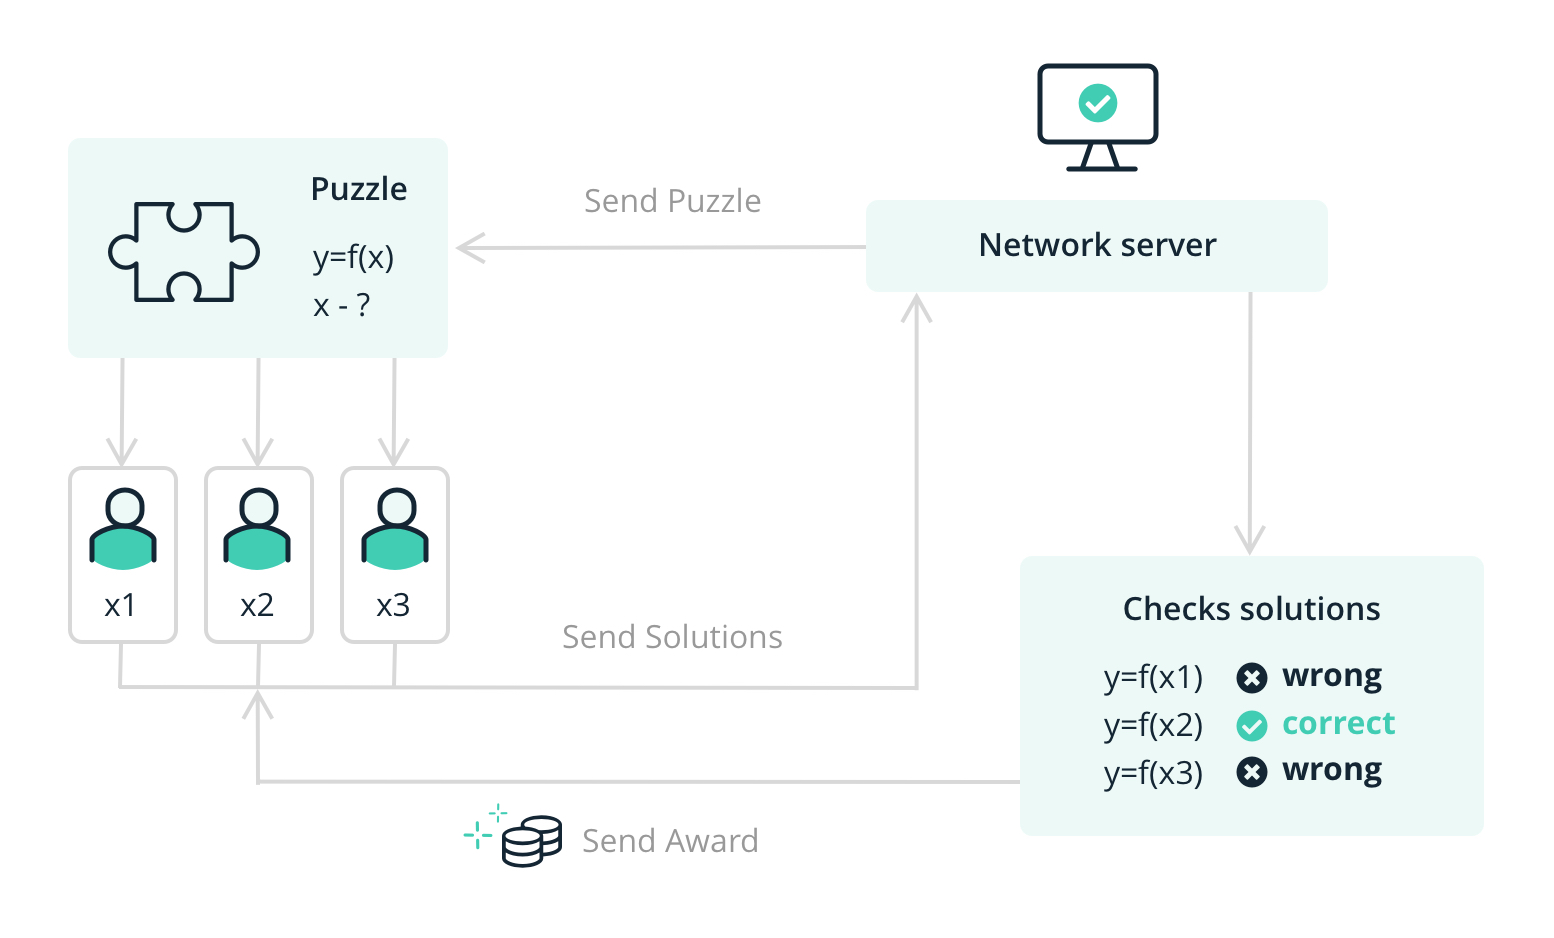
\includegraphics[width=0.65\textwidth]{Immagini/proof of work scheme.jpg}
\end{figure}
\\
Nell’ambito blockchain si sente spesso parlare di fork \cite{Blockchain_tecnologia_e_applicazioni_per_il_business}, ma non è sempre chiaro cosa si intenda con fork e cosa effettivamente comporti. Sebbene il termine venga spesso utilizzato per indicare la divisione di una blockchain in realtà esso racchiude un insieme di diversi possibili scenari. 
Una fork è una situazione in cui accade una delle seguenti cose:
\begin{itemize}
\item Può accadere che due o più nodi trovino contemporaneamente una soluzione valida. In tal caso, si generano due blocchi con lo stesso genitore, creando una biforcazione nella catena, detta fork. Quando viene individuato il blocco successivo, l’algoritmo seleziona la catena più lunga (in termini di difficoltà complessiva) come valida. Questo caso viene denominato come fork regolare.
\item Le regole della Blockchain sono cambiate in maniera retrocompatibile e tutti i nodi condividono la stessa cronologia delle transazioni, in questo caso si tratta di soft fork e non c’è una divisione della blockchain.
\item Le regole della Blockchain sono cambiate in maniera non retrocompatibile, ma tutti i nodi si aggiornano alle nuove regole e condividono la stessa cronologia delle transazioni, anche in questo caso non si ha una divisione della blockchain, ma si tratta di un hard fork.
\item Le regole della blockchain sono cambiate in maniera non retrocompatibile e nodi diversi hanno opinioni diverse sulle regole della blolckchain, non condividendo la stessa cronologia delle transazioni, abbiamo quindi un hard fork con chain split, perchè avviene una divisione della chain e il consenso sulla cronologia delle transazioni e perso definitivamente.
\end{itemize}
Questo criterio, basato sul "principio di maggior lavoro", permette a tutti i nodi di concordare su una versione univoca della blockchain e di risolvere le biforcazioni. Un blocco viene considerato finalizzato quando sono stati generati almeno sei blocchi successivi. Questo livello di profondità rende economicamente insostenibile, per una minoranza di nodi malintenzionati, modificare i dati della blockchain, poiché richiederebbe un effort computazionale estremamente elevato pari al 51\% della potenza totale di calcolo del network e anche se ipoteticamente un miner riuscisse a raggiungere tale potenza non sarebbe comunque in grado di modificare le vecchie transazioni, poiché dovrebbe ricalcolare la PoW di tutti i blocchi successivi, mentre gli altri miner onesti continuano a minare sulla blockchain corretta. Un attacco di questo tipo richiederebbe l’utilizzo di una quantità incredibile di risorse per l’attacker. Se qualcuno effettivamente riuscisse a mettere insieme più del 51\% della potenza di calcolo, sarebbe molto più redditizio per lui seguire le regole della blockchain.
Nonostante i numerosi vantaggi che il Proof of Work offre, questo algoritmo di consenso presenta alcune significative criticità. La principale è il massiccio consumo di energia, un aspetto che, paradossalmente, costituisce anche uno dei suoi punti di forza, rendendo estremamente costoso e complesso attaccare la rete.
A questo si aggiunge la scarsa scalabilità del sistema, che si traduce in una certa lentezza nell’elaborazione delle transazioni e nell’aumento delle commissioni, soprattutto nei periodi di maggiore attività sulla rete. Infine, il Proof of Work tende a creare una sorta di discriminazione geografica: attualmente, la maggior parte dei miner si concentra in aree dove il costo dell’elettricità è più basso, limitando la partecipazione globale e accentuando disparità economiche e infrastrutturali.

\section{Blokchain 2.0}

\subsection{Ethereum e Proof Of Stake}
Bitcoin, per sua natura, non è stato concepito come un ambiente di sviluppo e offre funzionalità di programmazione molto limitate, mentre la community ha sempre voluto mantenere la piattaforma focalizzata sullo scambio di valori, lasciando spazio a progetti alternativi che miravano ad ampliare le possibilità della tecnologia blockchain.
È in questo scenario che nasce Ethereum, la prima blockchain progettata specificamente per supportare lo sviluppo di applicazioni decentralizzate. Co-fondata nel 2013 da Vitalik Buterin, un programmatore russo-canadese che in passato aveva collaborato con Bitcoin Magazine, Ethereum si distingue da Bitcoin per molteplici innovazioni.
Una delle principali novità introdotte è la possibilità di utilizzare due tipi di conti: i tradizionali conti posseduti tramite una coppia di chiavi pubblica e privata, come in Bitcoin, e i conti associati agli Smart Contract \cite{Blockchain_guida_allecosistema}. Gli Smart Contract, concettualizzati per la prima volta da Nick Szabo nel 1994, sono programmi in grado di eseguire automaticamente azioni predeterminate una volta soddisfatte certe condizioni.
Questi contratti decentralizzati garantiscono che le regole siano rispettate senza la necessità di intermediari, eliminando possibili interferenze.
Un esempio pratico di utilizzo degli Smart Contract è il crowdfunding. Un utente potrebbe pubblicare un progetto stabilendo un obiettivo economico e un tempo limite per raggiungerlo. Lo Smart Contract, in questo caso, si occuperebbe di raccogliere i fondi dagli investitori e trattenerli fino al completamento della campagna. Se l’obiettivo viene raggiunto, i fondi vengono trasferiti automaticamente al creatore del progetto; in caso contrario, tornano ai donatori. Questa struttura elimina la necessità di intermediari e rende il processo completamente trasparente.
Ethereum utilizza Solidity, un linguaggio di programmazione simile a JavaScript, per scrivere Smart Contract. La flessibilità offerta da questa piattaforma ha rivoluzionato il mondo delle blockchain, permettendo la creazione di applicazioni decentralizzate e inaugurando l’era delle cosiddette blockchain 2.0.
Inizialmente veniva utilizzato il meccanismo di consenso Proof of Work (PoW), lo stesso di Bitcoin, però per migliorare efficienza e sostenibilità, il 15 settembre 2022, con l’aggiornamento noto come The Merge, Ethereum è passato al Proof of Stake (PoS). 
Questo cambiamento ha segnato un cambio epocale per la piattaforma ed ha portato con se enormi vantaggi.
Il PoS riduce drasticamente il consumo energetico, abbassandolo del 99,9\% rispetto al PoW, ed elimina la necessità di hardware costoso per il mining, rendendo la partecipazione al consenso più accessibile.
Con l’introduzione del PoS, Ethereum ha reso possibile lo staking, un processo in cui i partecipanti bloccano una quantità di criptovaluta in uno Smart Contract per sostenere la sicurezza e il funzionamento della blockchain. Attraverso lo staking, gli utenti possono diventare validatori e partecipare attivamente alla convalida delle transazioni e alla creazione di nuovi blocchi.
Lo staking offre numerosi vantaggi: aumenta la sicurezza del sistema rendendo gli attacchi costosi e difficili da eseguire, favorisce la decentralizzazione permettendo a più utenti di contribuire alla rete e riduce il consumo energetico rispetto al mining tradizionale. I partecipanti allo staking ricevono ricompense proporzionali alla loro attività, sotto forma di nuove criptovalute o una parte delle commissioni generate dalle transazioni.
Le ricompense non si limitano ai validatori che propongono nuovi blocchi, ma includono anche coloro che verificano e confermano la validità dei blocchi proposti da altri. Questo sistema rende lo staking una delle principali motivazioni per partecipare al consenso su Ethereum, favorendo un equilibrio tra efficienza e incentivi economici.
Inoltre, il sistema garantisce una maggiore scalabilità e permette ai validatori onesti di proteggere la rete da attacchi, penalizzando economicamente i nodi malevoli o inattivi per almeno il 50\% del tempo attraverso un meccanismo chiamato slashing che risulterà totale per i primi andando a sottrarre in maniera permanente le risorse depositate nello stake, mentre sarà parziale per i secondi che si vedranno sottratti solo i guadagni ricevuti ma non saranno rimossi dalla chain.
Nonostante questi vantaggi, il PoS presenta alcune criticità. Essendo una tecnologia più recente rispetto al PoW, è meno testata e potrebbe essere più vulnerabile a eventi imprevisti, i cosiddetti Black Swan. Inoltre, il fatto che il controllo della rete sia legato al possesso di criptovalute pone un rischio di centralizzazione: chi dispone di maggiori capitali potrebbe accumulare una quantità significativa di token, aumentando la propria influenza sul sistema.

    \chapter{Sicurezza}
\section{Privacy e sicurezza}
L'adozione delle tecnologie basate sulla blockchain  si è progressivamente ampliata oltre il settore delle criptovalute, trovando applicazione in ambiti importanti come quello della protezione della privacy \cite{borroni_blockchain_2019}.
\\La spinta verso la decentralizzazione deriva principalmente dalle crescenti preoccupazioni degli utenti riguardo alla perdita di controllo sui propri dati personali archiviati online \cite{rodota_quattro_paradigmi_2018} \cite{alpa_identita_digitale_2017}.
\\A tal riguardo, la struttura stessa della blockchain offre potenzialità per tutelare la riservatezza delle informazioni personali; tuttavia l'analisi dei metadati può renderla vulnerabile in determinati contesti. 
\\Di conseguenza, senza un'adeguata progettazione,
«\textit{decentralized infrastructures intended to promote individual privacy and autonomy might turn out to be much more vulnerable to governmental or corporate surveillance than their centralized counterparts}» \cite{de_filippi_interplay_2016}.
\\In questa prospettiva, non va dimenticato che la natura pseudonima di molte
reti che si basano sulla blockchain consente agli individui la possibilità di
condurre le proprie transazioni su base peer-to-peer, senza la necessità di
rivelare la propria identità alle controparti.

\subsection{Il difficile rapporto tra trasparenza e privacy}
Allo stesso tempo, la trasparenza derivante dalle distributed ledger technologies è tale che chiunque ha la possibilità di accedere alla
cronologia di tutte le transazioni memorizzate sulla blockchain, affidandosi così all’analisi dei dati in essa contenuti per ricavare informazioni potenzialmente sensibili \cite{marr_history_blockchain_2018}.
\\Se il sistema non viene progettato con la dovuta attenzione, la trasparenza potrebbe compromettere la tutela della privacy degli utenti, in quanto questi avrebbero
accesso ai dati di tutti gli altri utenti presenti sulla piattaforma e quindi si avrebbe un miglioramento della trasparenza 
a discapito però della privacy \cite{zambardino_blockchain_2022} \cite{mayes_privacy_transparency_2018}.\\
Pertanto in assenza di soluzioni tecniche adeguate per salvaguardare la riservatezza delle comunicazioni online, le infrastrutture decentralizzate, pensate per favorire privacy e autonomia, 
rischiano di risultare più esposte al controllo di governi o aziende rispetto ai sistemi centralizzati.
\\Resta comunque una notevole incertezza riguardo alla capacità di soluzioni alternative e decentralizzate di affrontare efficacemente le problematiche legate alla protezione dei dati.
\\Nonostante ciò, i sistemi decentralizzati, come la blockchain, hanno suscitato un crescente interesse nella comunità accademica che sta approfondendo il potenziale utilizzo delle DLTs in ambito privacy.
\\Per comprendere meglio le questioni legate alla protezione dei dati personali, è fondamentale esaminare due aspetti principali:
\begin{itemize}
    \item l'individuazione del soggetto responsabile della definizione delle modalità di trattamento dei dati personali;
    \item l'identificazione di chi controlla la conservazione e gestione dei dati.
\end{itemize}
La natura decentralizzata della blockchain non solo garantisce livelli più elevati di protezione dei dati personali, ma conferisce agli utenti un maggiore controllo sulle proprie informazioni, permettendo loro di gestirle autonomamente durante gli scambi. \\Questa tecnologia è stata infatti descritta dalla dottrina come un vero e proprio «\textit{sistema di cloud computing decentralizzato}» \cite{bridge_blockchain_2018}.
\\In tale contesto, il principale vantaggio offerto dai sistemi decentralizzati risiede nella possibilità per gli utenti di assumere un controllo diretto sulla gestione dei propri dati, inoltre le informazioni generate, condivise e raccolte dagli utenti stessi potrebbero essere messe a disposizione o vendute per fini comuni,
consentendo l'accesso anche a terze parti. Questo approccio ricorda quello degli open data, ma con meccanismi e logiche significativamente diversi.
\\Per quanto riguarda la struttura, gran parte delle architetture decentralizzate disponibili per gli utenti sono progettate con l'obiettivo di favorire la privacy, focalizzandosi su almeno uno dei due paradigmi fondamentali: la riservatezza dei dati e la “sovranità” su di essi.
\\In questa prospettiva, la decentralizzazione che caratterizza la blockchain offre un potenziale significativo per ridurre le asimmetrie informative che si verificano quando una delle parti coinvolte in una transazione possiede informazioni rilevanti che l'altra parte non conosce, le quali, nei sistemi centralizzati, tendono a creare vantaggi per gli operatori a discapito degli utenti.
\\Tuttavia va evidenziato che, allo stato attuale, persistono numerose complessità nel comprendere appieno come privacy e trasparenza possano interagire tra loro.
\\In una società “trasparente”, qualsiasi parte interessata può facilmente accedere alle informazioni, questo implica che la trasparenza sociale possa compromettere il diritto alla privacy. \`E legittimo quindi associare una crescente trasparenza delle informazioni a un ridotto rispetto del diritto alla privacy.
\\In tale contesto la trasparenza offerta dalle DLTs non è né totale né incondizionata. 

\subsection{Blockchain permissioned e permissionless}
Le diverse tipologie di blockchain, infatti, possono garantire vari livelli di trasparenza. Esistono, in particolare, due tipologie di blockchain: 
\begin{itemize}
    \item[\textbullet\ \textit{permissioned} $\rightarrow$] in cui una sola autorità ha il permesso di scrivere sulla blockchain e detiene praticamente il controllo del sistema distribuito;
    \item[\textbullet\ \textit{permissionless} $\rightarrow$] in cui chiunque può partecipare come nodo, verificare transazioni e aggiungere blocchi al registro, tutti i dati delle transazioni sono visibili e accessibili a chiunque abbia accesso alla rete, anche se non tutti possono necessariamente scrivere nella blockchain (ma chiunque può leggere i dati).
\end{itemize}
Soprattutto nel caso delle blockchain permissioned, le transazioni (o scambi, scrittura delle informazioni) avvengono all’interno di un ecosistema chiuso, dove i dati registrati sono mantenuti riservati e le identità dei partecipanti sono note \cite{Blockchain_tecnologia_e_applicazioni_per_il_business}.
\subsection{Crittografia End-to-End e responsabilità degli algoritmi}
Da un punto di vista pratico, i problemi di privacy legati al livello di trasparenza della blockchain possono essere attenuati mediante la crittografia “end-to-end” delle comunicazioni che utilizza chiavi private e pubbliche, anziché una chiave unica per crittografare e decrittografare.
\\Il principio implica che, ove possibile, le operazioni del protocollo di comunicazione debbano essere eseguite ai punti finali di un sistema di comunicazione, il più vicino possibile alla fonte o al destinatario finale dei dati, o comunque alla risorsa da controllare.
\\In particolare, le aspettative sociali riguardo la trasparenza e la supervisione degli algoritmi sono in forte crescita, con l’obiettivo di rendere i sistemi decisionali automatizzati sempre più responsabili, trasparenti e governabili. 
\\Si sta cercando di dotare questi sistemi di nuovi strumenti tecnologici, per verificare che le decisioni automatizzate rispettino standard di equità giuridica. 
\\Garantire la responsabilità, attraverso valutazioni d’impatto degli algoritmi (AIA) \cite{reisman_algorithmic_2018}, audit e certificazioni dovrebbe diventare parte integrante delle iniziative politiche e legali in questo ambito, considerando che la blockchain, al momento, non è stata ancora completamente implementata \cite{zhang_end_to_end_3}.

\section{Web 3.0}
L'idea del Web 3.0 è stata inzialmente utilizzata in stretta connessione con il concetto di web semantico, terminologia creata da Berners Lee in un articolo di \textit{Scientific American} del 2001 per descrivere un nuovo web. 
La sua idea è che, così come il web 2.0 permette di collegare pagine web a livello di visualizzazione, il web semantico deve permettere non solo di collegare pagine tra loro ma anche i dati contenuti in esse \cite{ted_youtube}.
\\La visone del web semantico è una visione di dati interconnessi e navigabili che possono essere usati da chiunque. L'esigenza di socializzazione dei dati è ancora più importante oggi poiché l'intelligenza artificiale può costruire modelli a partire dai dati grezzi, sulla base di algoritmi generali.
\\L'obiettivo del web 3.0, riconosciuto da Gavin Wood, co-fondatore di Ethereum, è quello di creare un web decentralizzato, dove i dati sono posseduti dagli utenti e non da poche aziende. Sta nascendo la consapevolezza di re-decentralizzare i servizi web \cite{Blockchain_tecnologia_e_applicazioni_per_il_business}.
\\Questa idea è diffusa da molto tempo, ma adesso finalmente esistono le tencologie che permettono di realizzarla, come la blockchain 
e così si potrebbero ottenere numerosi vantaggi, tra i quali:
\vspace{1em}
\begin{adjustwidth}{2cm}{0pt}
    \begin{itemize}[itemsep=1ex]
        \item [\textbullet\ \textit{decentralizzazione} $\rightarrow$ ] non è necessario alcun permesso da parte di un'autorità centrale per caricare qualcosa sul web. Questo fornisce una protezione contro qualsiasi forma di censura e controllo e il web tornerebbe ad essere un sistema neutrale;
        \item [\textbullet\ \textit{democratizzazione} $\rightarrow$ ] è possibile offrire un accesso a chiunque abbia una connessione a internet, senza discriminazioni su età, sesso, razza, religione e posizione geografica;
        \item [\textbullet\ \textit{uptime dei servizi} $\rightarrow$ ] non essendoci nodi centrali, non esiste un punto di fallimento. Se un nodo va giù, il servizio rimane comunque disponibile;
        \item [\textbullet\ \textit{possesso dei dati} $\rightarrow$ ] gli utenti riprenderebbero possesso dei propri dati potendo decidere con chi condividerli e in che modo.
        \\Inoltre potrebbero potenzialmente anche guadagnarci dalla vendita di quest'ultimi attraverso smart contracts effettuati con le grandi multinazionali, come FaceBook e Google. Le quali poi le cedono agli advertiser che pagano milioni per avere questi dati;
        \item [\textbullet\ \textit{persistenza dei dati} $\rightarrow$ ] i dati non possono essere cancellati, a meno che non venga cancellata l'intera blockchain, questo perchè vengono salvati in maniera ridondante su diversi nodi distribuiti indipendentemente.
    \end{itemize}
\end{adjustwidth}
\vspace{1em}

\begin{figure}[h]
    \caption{Livelli del web 3.0}
    \centering
    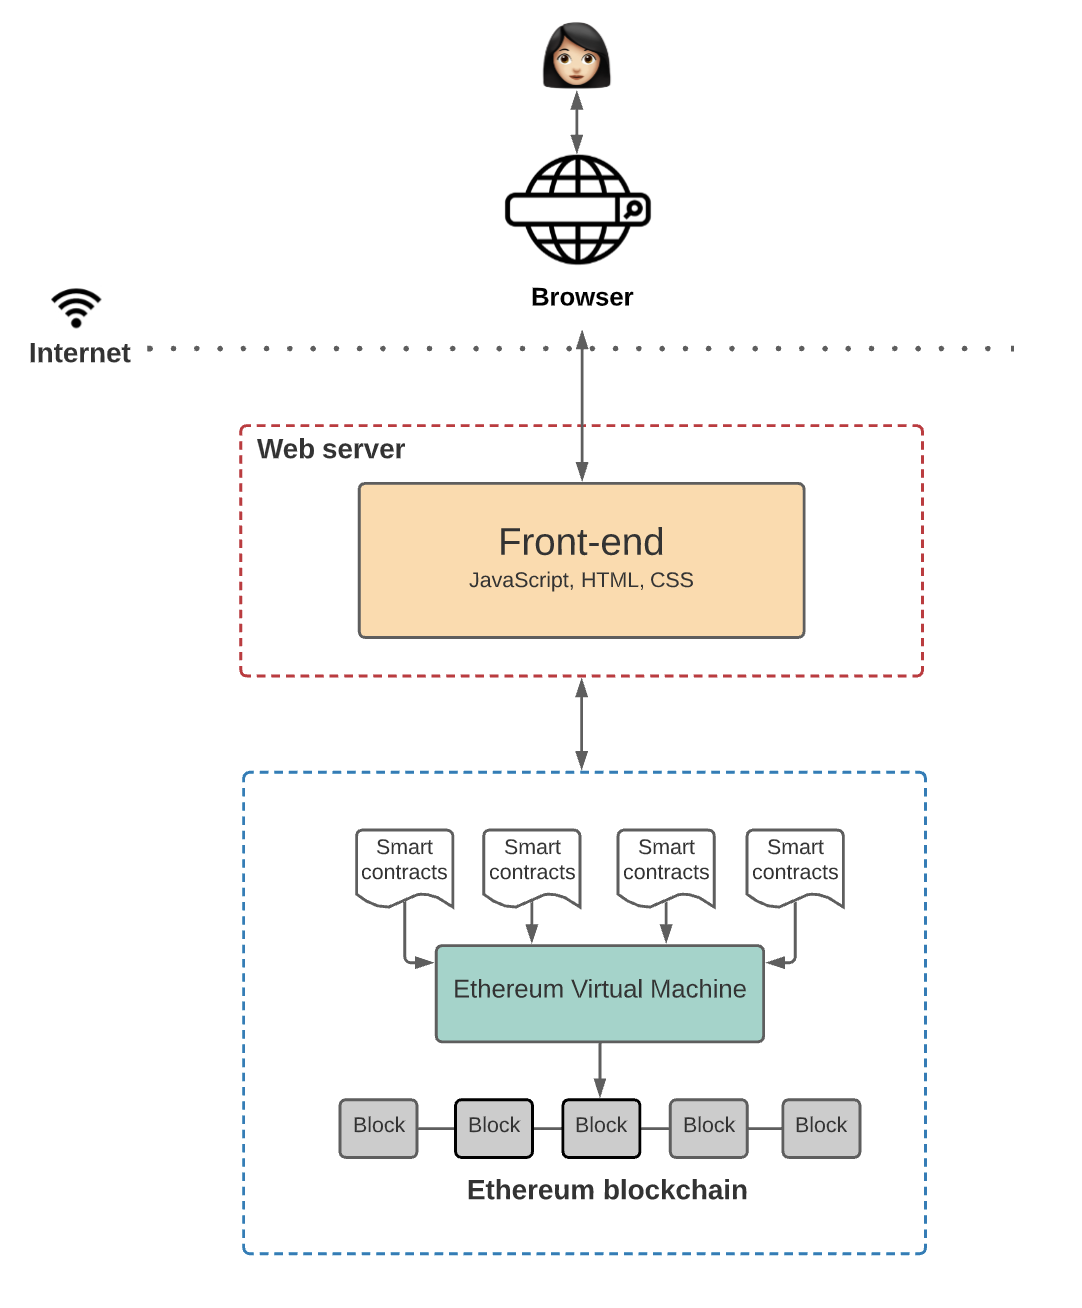
\includegraphics[width=0.65\textwidth]{Immagini/web_30.png}
\end{figure}
L'architettura del web 3.0 non è ancora stata definita in maniera chiara e ufficiale, ma la sua caratteristica chiave sarà certamente l'assenza
di divisione netta tra utenti e fornitori di servizi. Per esempio quando ci colleghiamo a FaceBook siamo utenti e quest'ultimo agisce come provider 
offrendoci un servizio in cambio dei nostri dati personali. 
\\La prossima iterazione del web permetterà di eliminare questa contrapposizione netta, perchè
gli utenti potranno essere anche fornitori di servizi, almeno nelle Blockchain permissionless \cite{Blockchain_guida_allecosistema}.

    \chapter{Learning Analytics}
\section{Cos'è il Learning Analytics}
La delicata tematica di privacy e sicurezza affrontata nel capitolo precedente, caratterizza fortemente il ramo
del Learning Analytics.
\begin{wrapfigure}{r}{0.25\textwidth}
    \centering
    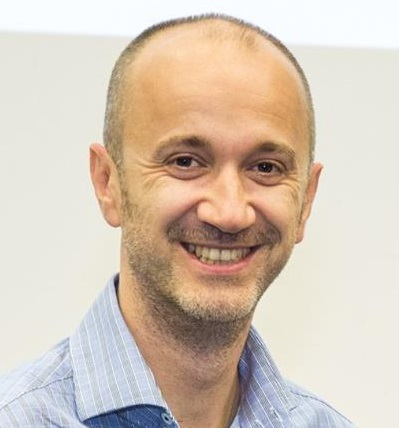
\includegraphics[width=0.25\textwidth]{Immagini/Dragan Gasevic.jpg}
    \caption{Dragan Gasevic}
    \subcaption{Padre di Learning Analytics}
\end{wrapfigure}
Questo particolare campo emergente nell'ambito dell'educazione si concentra nel raccogliere, misurare e analizzare i dati raccolti sugli studenti e sui loro corsi
di studio, con l'obiettivo di ottimizzare l'esperienza educativa e migliorare non solo i loro risultati, ma anche i metodi di insegnamento. 
\\Grazie alla crescente digitalizzazione e all'adozione di strumenti 
come i Learning Management System (LMS), i social media e i corsi online aperti e massivi (MOOCs), è possibile raccogliere una grande quantità di dati relativi al comportamento degli studenti, 
ai loro risultati e alle interazioni con i materiali didattici. 
\\Il Learning Analytics offre un enorme aiuto a tutti gli stakeholder coinvolti nel processo educativo:
\begin{itemize}
    \item Agli studenti che possono riflettere sui propri progressi e migliorare il proprio apprendimento attraverso feedback personalizzati e a loro volta dare feedback sui corsi per aiutare i docenti a migliorare i metodi di insegnamento.
    \item Ai docenti che possono adattare i contenuti dei corsi in base ai feedback e ai risultati degli studenti e identificare tempestivamente gli studenti in difficoltà.
    \item Agli amministratori accademici che possono utilizzare i dati per prendere decisioni basate sull'evidenza e sviluppare strategie efficaci per migliorare l'efficienza e la qualità dell'istruzione.
\end{itemize}
Proprio per questo le principali applicazioni del Learning Analytics sono il monitoraggio delle prestazioni individuali, la prevenzione dell'abbandono scolastico,
la personalizzazione dei percorsi educativi e l'analisi delle tecniche di valutazione e dei curricula \cite{wikipedia_learning_analytics}.

\section{Limiti del Learning Analytics}
Nonostante la disponibilità di standard di riferimento per la gestione dei dati di apprendimento su un LRS (Learning Record Store), è ancora difficile raggiungere l'interoperabilità,
ovvero la capacità di due piattaforme differenti di scambiare le informazioni in maniera indipendentemente, senza alcune limitazioni.
\\Questi problemi includono:
\begin{itemize}
    \item Collegare le storie di apprendimento di uno studente su diverse piattaforme di apprendimento in un unico percorso immutabile, in modo tale che ogni studente abbia un'unica identità nel web e non diverse identità in base alle piattaforme su cui si collega.
    \item Garantire la privacy dei registri degli studenti con facilità nel controllo degli accessi.
    \item Integrare i sistemi di ricerca e produzione per migliorare l'apprendimento.
\end{itemize}

\subsection{Collegare le storie di apprendimento }
Sebbene gli studenti spesso passino da una piattaforma di apprendimento di un provider a un'altra, i loro record di apprendimento vengono memorizzati separatamente in LRS distinti e in modo disconnesso. 
Di conseguenza, ogni sistema deve sostenere il costo di ricostruire i dati dell'apprendente da zero anche per casi molto semplici. Anche se questo potrebbe non rappresentare uno sforzo ripetuto per i principianti, è quasi impossibile determinare se uno studente sia realmente un principiante.
Questo causa anche un problema di "\textit{cold start}" nei sistemi di raccomandazione per la formazione, a causa della mancanza di azioni di apprendimento precedenti degli studenti \cite{barnes_stamper_2008}.
I sistemi proposti dovrebbero consentire agli studenti di portare con sé i propri dati di apprendimento,
nello stesso modo in cui possono facilmente trasferire i certificati da un'istituzione all'altra. 
\\A tal proposito tornerebbe utile il design del Web 3.0 presentato nel capitolo precedente che permetterebbe a ogni studente di costruirsi un'identità digitale univoca indipendente dal provider di servizi e che consentirebbe di
andare a risolvere il problema di cold start, in quanto non servirebbe più ricostruire ogni volta la storia di apprendimento di uno studente, ma basterebbe andare a leggere la sua identità digitale \cite{ocheja2018connecting}.

\subsection{Privacy, sicurezza e controllo degli accessi}
Questo è un altro problema quando si condividono i risultati di apprendimento individuali degli studenti con terze parti. 
\\Sebbene l'analisi dell'apprendimento aiuti a migliorare le prestazioni degli studenti, attraverso una domanda generale e quattro specifiche sulle condizioni per la privacy degli studenti, sostengono che, qualunque siano i guadagni dalle analisi dell'apprendimento, questi devono tener conto sempre al rispetto della privacy e dei diritti degli studenti,
quindi non si potrà andare a violare la privacy dello studente per avere una maggiore efficienza dalle analisi dell'apprendimento,
questo perchè il trauma psicologico che potrebbe derivare da una singola violazione della privacy può essere devastante, poiché è possibile rivelare informazioni riservate e dunque sensibili. 
\\I sistemi proposti devono quindi garantire in primis la priorità al rispetto alla privacy degli studenti, lasciando a loro il controllo decisionale dei propri dati di apprendimento \cite{ocheja2018connecting}.

\subsection{Integrare i sistemi di ricerca e produzione}
La disponibilità di dati di apprendimento per la ricerca favorisce l'innovazione. 
Nei casi in cui i dati di apprendimento siano raccolti da sistemi di produzione e/o di ricerca, i ricercatori di learning analytics spesso si trovano a dover affrontare il difficile compito di anonimizzare le informazioni personali con lo scopo di mantenere protetta la privacy degli stakeholder, facendo così si ha però un'immensa dispersione di risorse impiegate nel processo di anonimizzazione e inoltre si ha un impatto negativo sui risultati, perchè si va a perderne la loro caratterizzazione e personalizzazione. 
\\Poiché i dati di apprendimento in tempo reale diventano sempre più desiderabili per la ricerca in learning analytics, è cruciale sviluppare nuove idee su come integrare in modo fluido e interoperabile i sistemi di ricerca e produzione, garantendo al contempo la privacy di tutti gli stakeholder coinvolti \cite{ocheja2018connecting}.

\section{Blockchain come soluzione}
Ogni stakeholder deve quindi avere diritti diversi sui dati e metadati, 
di conseguenza, i dati devono essere circondati da diversi livelli di accesso degli utenti, ciascuno con permessi specifici e unici,
in modo tale che gli studenti possano avere accesso solamente ai loro dati, gli insegnanti ai dati di tutti i loro studenti, mentre i genitori solo ai dati relativi ai propri figli.
\\La natura di questi diritti e il modo in cui vengono applicati devono essere concordati in modo esplicito e chiaramente comprensibile da tutti, 
inoltre potrebbero essere validi solo per periodi di tempo limitati e vincolati al soddisfacimento di determinate condizioni, in modo tale da garantire un'adeguata anonimizzazione dei dati per rispettare la privacy di ciascun stakeholder.
\\Ha quindi senso archiviare tutti i dati e metadati relativi allo studente rilevanti per le Learning Analytics in un decentralized distributed ledger basato su un sistema Blockchain \cite{Learning_Analytics_Privacy_on_the_Blockchain}.
\\Grazie a questo sistema si potranno andare a soddisfare i seguenti requisiti:
\begin{itemize}
    \item[\textit{Autenticità}:] I "\textit{Data and metadata About Learning Processes}" (DALP) avranno la prova di essere validi e di essere stati aggiunti da utenti autorizzati, questo è molto importante perchè dire "\textit{Uno studento sostiene di aver preso un 30 all'esame}" non è la stessa cosa di dire "\textit{L'insegnante sostiene che lo studente abbia preso 30}".
    \item[\textit{Integritàtà}:] I dati non potranno essere modificati.
    \item[\textit{Controllo}:] Solo gli stakeholder autorizzati avranno il diritto di accedere ai dati, ma solo ai dati che gli corrispondono. 
    \item[\textit{Conoscenza}:] Verrà sempre tenuto traccia sul registro di chi ha acceduto ai dati e il motivo per cui lo ha fatto.
    \item[\textit{Sicurezza}:] I dati saranno protetti da furti e attacchi informatici, grazie al design della Blockchain.
\end{itemize}
\'E facile notare come la nascita di una piattaforma che necessita questi requisiti sarebbe molto più spontanea e naturale e meno costosa se 
fosse inserita in un ecosistema che la favorisse soddisfandone già a sua volta i requisiti, è importante quindi evidenziare ancora una volta
l'importanza che avrebbe il passaggio del web da 2.0 a 3.0 e gli innumerevoli vantaggi che ciò porterebbe.
\\Nei paragrafi che seguiranno vedremo nel dettaglio alcuni esempi tangibili di piattaforme Blockchain-based nell'ambito educativo che sono al momento dispobili sul web.
\section{EduCTX}
La più importante piattaforma nel settore educativo basata su Blockchain è EduCTX, sviluppata da un consorzio di università europee sfrutta la Blockchain 2.0 di Ethereum con lo scopo di gestire i crediti e le valutazioni nell'istruzione superiore.
\\In ambito di Learning Analytics è molto importante l'apporto di EduCTX, in quanto permette di raccogliere i certificati e i risultati degli studenti sui quali effettuare le analisi.
\\Al momento questa piattaforma presenta due versioni, la versione 1.2 sulla quale noi focalizzeremo il nostro interesse in quanto costruita su Blockchain
sfruttando il portale di registrazione MetaMask e la versione 2.0 che invece si basa su Microsoft Azure Active Directory un servizio di gestione d'identità centralizzato basato su cloud.
\begin{figure}[h]
    \centering
    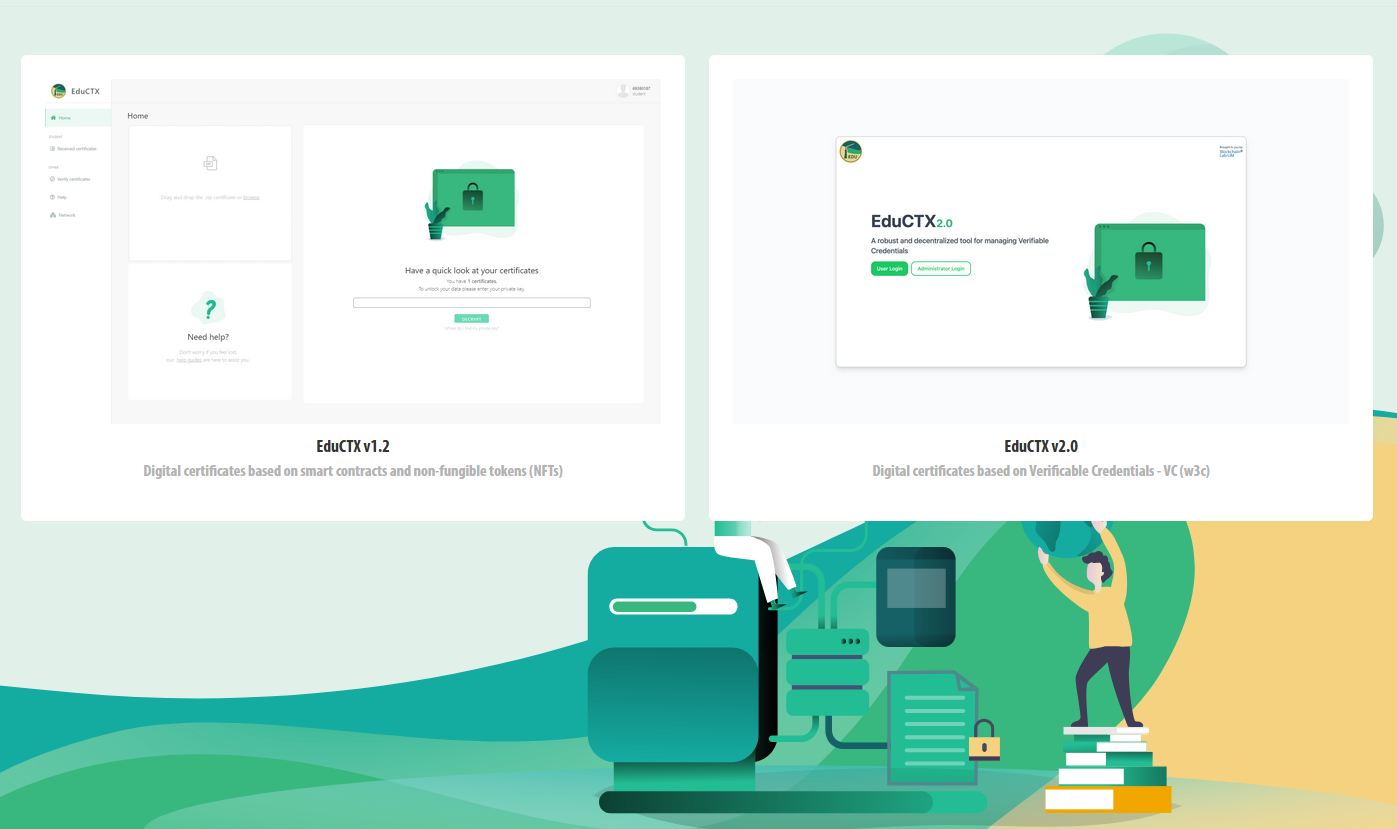
\includegraphics[width=0.85\textwidth]{Immagini/EduCTX.PNG}
    \caption{EduCTX homepage}
\end{figure}

\subsection{Struttura}
La piattaforma EduCTX è concepita per elaborare, gestire e controllare i token ECTX come crediti accademici, basandosi su una rete P2P globalmente distribuita, 
in cui i nodi della rete blockchain sono gli istituti di istruzione superiore (HEI), mentre gli utenti della piattaforma sono studenti e organizzazioni.
\\I token ECTX rappresentano l’equivalente del valore dei crediti ottenuti dagli studenti per i corsi completati.
\\Ogni studente disporrà di un portafoglio blockchain dedicato sulla piattaforma EduCTX, in cui potrà raccogliere i token ECTX, ossia il valore dei crediti assegnati dall’HEI per i corsi completati. 
\\Ogni volta che uno studente completa un corso, l’HEI di appartenenza trasferirà il numero appropriato di token ECTX al suo indirizzo blockchain. 
\\Le informazioni sul trasferimento vengono archiviate sulla blockchain, 
includendo i seguenti dati: 
\begin{itemize}
    \item il mittente, identificato come l’HEI con il suo nome ufficiale.
    \item il destinatario, presentato in modo anonimo.
    \item il token - valore del credito del corso.
    \item l’identificazione del corso.
\end{itemize}
Inoltre, utilizzando il proprio indirizzo blockchain, lo studente, in qualità di destinatario dei token ECTX, può dimostrare globalmente i corsi completati, senza ostacoli amministrativi, di traduzione o linguistici, semplicemente presentando il suo indirizzo blockchain. 
\\Per garantire la sicurezza, agli studenti viene assegnato un indirizzo con firma multipla 2-2 da parte dell’HEI di appartenenza, impedendo loro di trasferire i token ECTX guadagnati verso altri indirizzi. 
\\Il processo di assegnazione dei token ECTX agli studenti e la loro capacità di dimostrarne il possesso sono gestiti tramite un client API blockchain EduCTX facile da usare che rende l’utilizzo della piattaforma il più intuitivo possibile.
\begin{figure}[h]
    \centering
    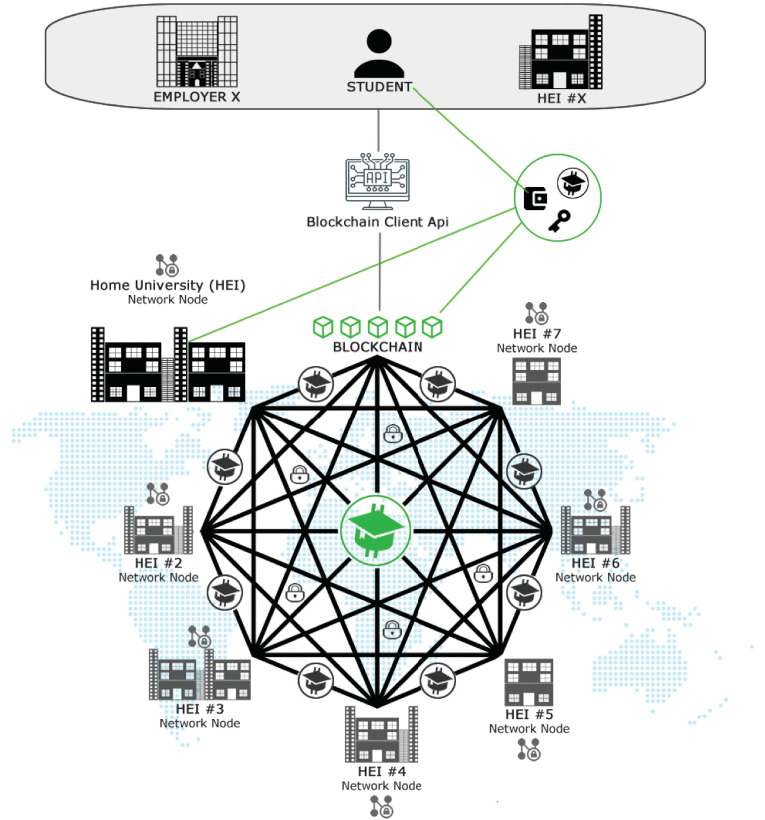
\includegraphics[width=0.65\textwidth]{Immagini/EduCTX_blockchain_structure.jpg}
    \caption{EduCTX struttura blockchain}
\end{figure}

\subsection{Registrazione degli HEI}
Qualsiasi HEI accreditato e i suoi membri potranno entrare a far parte della rete. 
Per aderire, l’HEI dovrà configurare un nodo di rete per mantenere un’infrastruttura globale e una rete sicura. 
Un nodo completamente funzionante trasmette messaggi attraverso la rete, primo passo del processo di transazione che porta alla conferma di un blocco, e quindi alla conferma del trasferimento dei crediti ECTX agli studenti per i corsi completati. 
Il nodo HEI include anche il client blockchain EduCTX principale nel proprio server, con la replica completa del registro blockchain. Questo aumenta la sicurezza, poiché un numero maggiore di nodi rende la rete più sicura.
Gli HEI, e quindi i nodi, non minano le transazioni, poiché la piattaforma blockchain EduCTX è basata sul protocollo di consenso DPoS. Pertanto, non è necessaria alcuna potenza di calcolo da parte del nodo HEI. 
Questo approccio è inoltre appropriato dal punto di vista della sicurezza per la rete EduCTX, poiché peer casuali non possono unirsi alla rete e generare nuovi token ECTX attraverso il mining. Di conseguenza, la blockchain EduCTX può essere considerata una versione consortile di una blockchain, ovvero una via di mezzo tra una blockchain permissioned e permissionless.
\\Ogni nuovo HEI che si unisce alla rete e viene verificato dagli altri membri HEI, riceve un’assegnazione iniziale di token ECTX e viene invitato a configurare un nodo di rete. Essendo una blockchain DPoS, ogni membro HEI può registrarsi come delegato nella piattaforma blockchain EduCTX e la comunità HEI vota un delegato che conferma le transazioni e sigilla i blocchi. 
Questo implica che la comunità vota per l’HEI più attivo e continuo nel suo lavoro. 
Per garantire una versione permissioned della piattaforma blockchain e una comunità democratica e senza scopo di lucro, la ricompensa per il forging è nulla \cite{EduCTX}.

\subsection{Registrazione degli studenti}
Quando uno studente si immatricola presso un HEI (membro della rete blockchain EduCTX), l'istituto emette un ID studente e genera un nuovo indirizzo blockchain per lo studente, contenente una chiave pubblica e una chiave privata
e anche un nuovo indirizzo blockchain con firma multipla 2-2 utilizzando la propria chiave pubblica e quella appena generata dello studente. 
\\Questo indirizzo con firma multipla, insieme all'ID studente, viene memorizzato nel database dell'HEI.
\\L'HEI trasferisce 0,1 token ECTX all'indirizzo blockchain con firma multipla 2-2 dello studente e, tramite un canale privato, fornisce allo studente le informazioni necessarie per configurare il portafoglio blockchain. 
\newpage
Le informazioni fornite includono:
\begin{itemize}
    \item Istruzioni per configurare un portafoglio blockchain EduCTX.
    \item L'indirizzo blockchain dello studente, contenente chiavi pubbliche e private.
    \item La chiave pubblica dell'HEI.
    \item Lo script di riscatto (redeem script).
\end{itemize}
Con le informazioni ricevute, lo studente configura il proprio portafoglio blockchain e un singolo indirizzo utilizzando le chiavi pubbliche e private fornite dall'amministrazione dell'HEI.
\section{Sony Global Education e Blockcerts}
Due importanti menzioni d'onore da fare nell'ambito dell'istruzione basata su Blockchain sono Sony Global Education e Blockcerts.
\\Entrando più nello specifico, Sony Global Education è a tutti gli effetti una piattaforma di Learning Analytics basata su una Blockchain permissioned sviluppata per l'appunto da Sony con l'obiettivo di raccogliere i dati 
sull'appredimento dei giovanissimi andando a migliorare il loro percorso di apprendimento, con un focus particolare sullo sviluppo della loro creatività.
\begin{figure}[h]
    \centering
    
\includegraphics[width=0.65\textwidth]{Immagini/Sony_Global_Education_logo.PNG}
    \caption{Sony Global Education Logo}
\end{figure}
\\Blockcerts è invece una piattaforma sviluppata dal MIT Media Lab in collaborazione con Learning Machine. 
\\Questa piattaforma è sullo stampo di EduCTX,
infatti può emettere certificati, o inoltre può permettere agli studenti di archiviare e verificare i loro certificati accademici, attestati professionali e altre credenziali.
In questo modo chiuque può verificare l'autenticità di un certificato senza dover contattare l'istituzione che lo ha rilasciato.
\\Questa piattaforma è basata su una Blockchain permissionless ed inizialmente è stata progettata per ancorare i certificati sulla blockchain di Bitcoin, 
ma successivamente ha iniziato a supportare Ethereum in modo tale da poter sfruttare gli Smart Contracts.
\newpage
\begin{figure}[h]
    \centering
    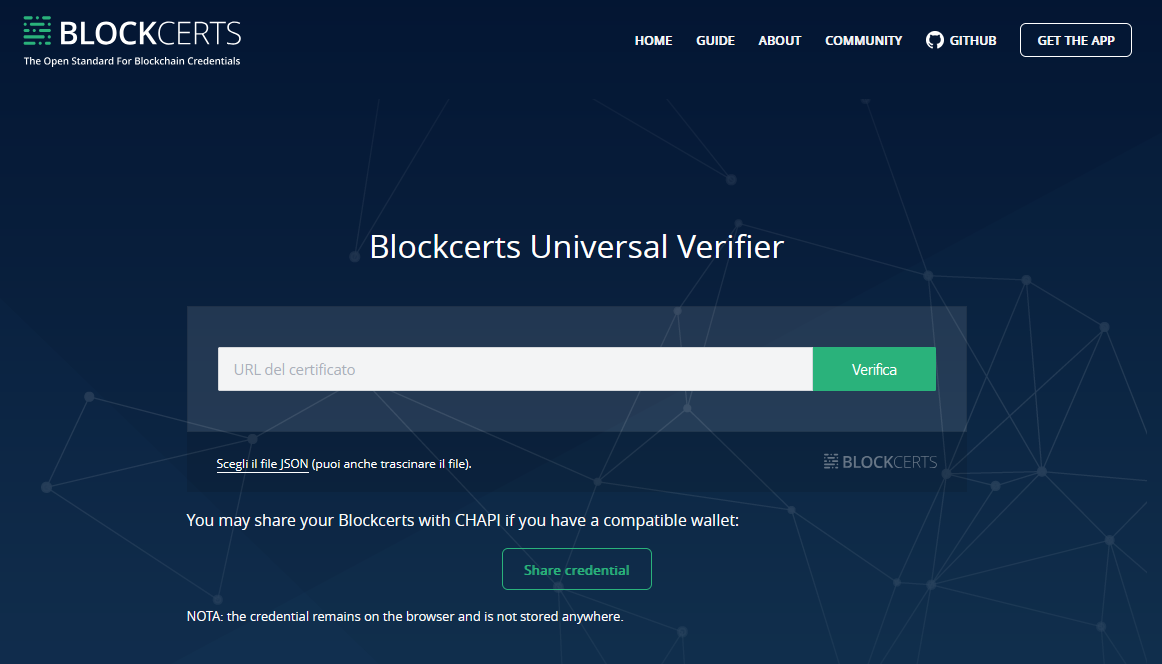
\includegraphics[width=0.65\textwidth]{Immagini/Blockcerts_homepage.PNG}
    \caption{Blockcerts homepage}
\end{figure}
Da fine 2019 Blockcerts è stata adottata anche dall'università di Padova, che ha iniziato a rilasciare i certificati di laurea in formato digitale scaricabli dalla piattaforma Bestr.

    \cleardoublepage
    \chapter{Conclusioni}
L'esigenza di capire e di prevedere l'evoluzione futura della società è sempre più presente e pressante,
in un mondo in cui la crescita esponenziale della tecnologia, di cui Blockchain è un esempio, ci costringe ad accelerare su una strada piuttosto tortuosa e piena di insidie.
\\Con la Blockchain abbiamo l'opportunità di digitalizzare istituzioni molto antiche, che fino ad oggi non hanno trovato un loro spazio online.
Ci ricordiamo di questo ogni volta che facciamo la fila agli uffici pubblici e ogni volta che votiamo con la matita sulla scheda elettorale.
\\Uno degli aspetti più significativi che ho appreso scrivendo questa tesi è che la blockchain non è una soluzione universale a tutti i problemi, ma piuttosto un nuovo paradigma che deve essere adottato con consapevolezza. 
Se da un lato offre strumenti potentissimi per decentralizzare il controllo e restituire agli utenti la proprietà dei propri dati, dall’altro solleva questioni di scalabilità, governance e sostenibilità energetica che devono essere affrontate con soluzioni mirate.
\\Come abbiamo visto, molte compagnie stanno già sfruttando la Blockchain per migliorare la trasparenza e la sicurezza, offrendo servizi che vanno a rispondere all'esigenza del mercato di avere un controllo maggiore sui propri dati.
\\L'istruzione è uno dei tanti settori che può trarre un enorme beneficio da questa tecnologia, in quanto la Blockchain può garantire la sicurezza e la trasparenza dei dati degli studenti, permettendo loro di avere un controllo maggiore sulle proprie informazioni e di poterle condividere con chi vogliono.
Sistemi come EduCTX, Sony Global Education e Blockcerts dimostrano che è possibile costruire un ecosistema più trasparente ed efficiente, in cui gli studenti possano avere pieno controllo sulle proprie informazioni e i certificati possano essere verificati in modo istantaneo e sicuro. 
\\La trasformazione blockchain-oriented della piattaforma FaceItTools, analizzata in questa tesi, di cui ho fornito una traccia da seguire prendendo spunto dai sistemi già presenti sul mercato è un esempio concreto di come questa tecnologia possa migliorare l’affidabilità e la privacy nel settore educativo.
\\Un'altra tematica che ho approfondito è il delicato equilibrio tra privacy e trasparenza. 
Se da un lato la blockchain offre una protezione dei dati più solida rispetto ai sistemi centralizzati, dall’altro è essenziale garantire che i meccanismi di accesso e autorizzazione siano adeguatamente progettati per evitare abusi e violazioni della privacy.
\\Proprio a tal proposito ho affrontato l'attuale stato di internet, dove gli utenti non sono in grado di controllare i propri dati e non sanno come vengono utilizzati, per questo motivo il passaggio al Web 3.0 porterebbe con sè innumerevoli novità segnando sicuramente una svolta epocale per la storia di internet per come lo conosciamo oggi.
\\Il vento di novità che soffia sopra questi argomenti è decisamente rinfrescante e pieno di senso di sfida che spinge a capire meglio l'impatto del cambiamento e come questo possa essere previsto e indirizzato.
\\Questa tesi cerca di racchiudere la maggior parte dei concetti più importanti, focalizzandosi sulla protezione della privacy dei dati personali e sulla trasparenza delle informazioni,
ma non può essere considerata una spiegazione esaustiva, in quanto l'argomento è estremamente vario e complesso. 
\\L'obiettivo è dunque quello di fornire uno spunto di partenza per altri studenti e ricercatori che vogliono approfondire l'argomento, proponendo delle implementazioni pratiche alle soluzioni proposte riguardo i problemi affrontati e a una possibile trasformazione blockchain-oriented della piattaforma FaceItTools, ma ricordando che l’innovazione tecnologica, per quanto avanzata, deve sempre essere accompagnata da un’etica solida e da una consapevolezza delle sue implicazioni sociali. 
La blockchain ha il potenziale per democratizzare l’accesso ai servizi digitali e ridurre le asimmetrie di potere, ma solo se utilizzata con responsabilità e con una visione che metta al centro gli utenti e la loro libertà.
    \cleardoublepage
    \printbibliography[heading=bibintoc]
\end{document}
